\documentclass[11pt]{article}

\usepackage{amsmath}
\usepackage{amsfonts}
\usepackage{amssymb}
\usepackage{xcolor}
\usepackage{graphicx}
\usepackage{bm}
\usepackage{mdframed}
\usepackage{mathtools}
\usepackage{empheq}
\usepackage{hyperref}
\usepackage{fullpage}
\usepackage[theorems,skins]{tcolorbox}

\hypersetup{
	colorlinks,
	citecolor=black,
	filecolor=black,
	linkcolor=blue,
	urlcolor=black
}

\title{The Frenet-Serret Frame}
\date{2021-01-12}
\author{Jay Khandkar}

\begin{document}

	\pagenumbering{gobble}
	\maketitle
	\newpage
	\tableofcontents
	\newpage
	\pagenumbering{arabic}
	
	\newcommand{\vect}[1]{\mathbf{#1}}
	\newcommand{\Mod}[1]{\lvert #1 \rvert}
	\newcommand{\ModFrac}[2]{\displaystyle\left\lvert \frac{#1}{#2} \right\rvert}
	\newcommand{\VectDiff}[1]{\dot{\vect{#1}}}
	\newcommand{\uveci}{{\bm{\hat{\textnormal{\bfseries\i}}}}}
    \newcommand{\uvecj}{{\bm{\hat{\textnormal{\bfseries\j}}}}}
    \newcommand{\uveck}{{\bm{\hat{\textnormal{\bfseries k}}}}}
    \newcommand*\widefbox[1]{\fbox{\hspace{2em}#1\hspace{2em}}}
    
	\begin{flushleft}
	
	\color{blue}
	\section{The TNB/Frenet-Serret Frame}
	\subsection{The Basis Vectors}
	\color{black}
	
	The TNB Frame,  or the Frenet-Serret Frame, is defined by the following vectors: 
	\begin{itemize}
		\item $\hat{T}$, the tangent unit vector,  which points in the direction of motion.
		\item $\hat{N}$, the normal unit vector.
		\item $\hat{B}$, the binormal unit vector,  the cross product of the tangent and normal vectors.
	\end{itemize}
	In further equations,  we shall drop the unit vector notation and represent vectors in boldface,  it is implied 
	that these vectors are of unit magnitude.  \\	
	
	\begin{figure}[h!]
     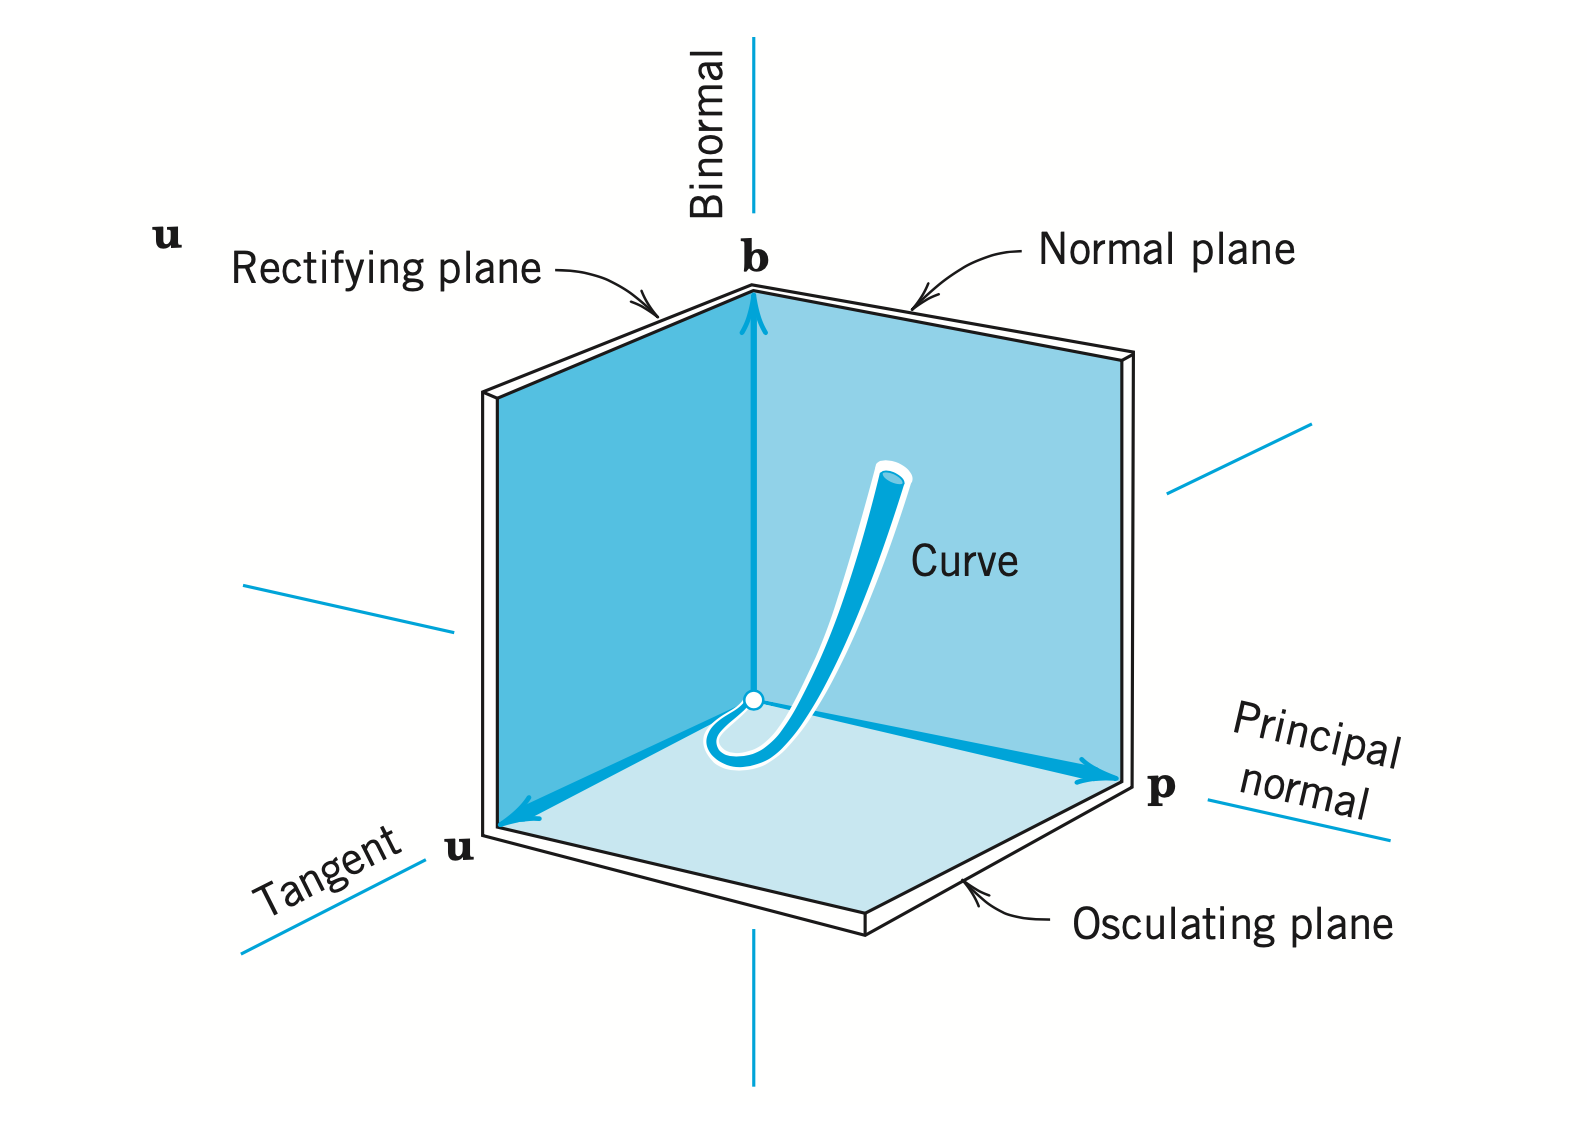
\includegraphics[width=\linewidth]{tnb.png}
     \caption{The Frenet-Serret Frame}
     \label{fig:boat1}
     \end{figure}
     The three unit vectors are defined as:\\
     \begin{align*}
     \vect{T} &= \frac{d\mathbf{r}}{ds}\tag{1}\\ 
     \\
     \vect{N} &= \frac{\frac{d\mathbf{T}}{ds}}{\ModFrac{d\vect{T}}{ds}\tag{2}}\\
     \\
     \vect{B} &= \mathbf{T}\times \mathbf{N}\tag{3}
     \end{align*}
     Here,  the variable $s$ is the arclength parameter,  given by 
     \begin{equation*}
     \boxed{\frac{ds}{dt} =\ModFrac{d\vect{r}}{dt} \tag{4}}
     \end{equation*}
     Henceforth,  we shall denote differentiation wrt.  the arbitrary parameter $t$ as $\mathbf{r'}$ and differentiation wrt. the 
     arclength $s$ as $\dot{\vect{r}}$.
    
    \color{blue}
     \section{The Curvature $\kappa$}
     \color{black}
   
     
     The curvature of a space curve $\vect{r}(t)$,  $\kappa$, gives a measure of how much it deviates from a straight line   at a particular point.  It is defined as
     
     \begin{equation*}
     \boxed{\kappa = \ModFrac{d\vect{T}}{ds} = \Mod{\dot{\vect{T}}} \tag{5}}
     \end{equation*}
     
     An analytical expression for $\kappa$ in terms of $\mathbf{r}$ and it's derivatives is obtained as follows:\\
     Using the chain rule, 
     
     \begin{align*}    
	\vect{r'} &= s'\dot{\vect{r}}\\\tag{6}
	\Rightarrow \vect{r''} &= s''\vect{T}+s'^{2}\dot{\vect{T}}
     \end{align*}
     
     Using $\kappa= \Mod{\dot{\vect{T}}}$ and $\mathbf{N} = \frac{\dot{\vect{T}}}{ \Mod{\dot{\vect{T}}}}$
     ,
     
     \begin{align*}
     \vect{r''} &= s''\mathbf{T}+s'^{2}\kappa\vect{N}\tag{7}
     \end{align*}
     
     Taking the cross product of $(6)$ and $(7)$,
     
     \begin{align*}
     \vect{r'} \times \vect{r''} &= s'\mathbf{T} \times s''\vect{T} + s' \kappa s'^{2}\vect{T} \times \vect{N}\\
     \Rightarrow \vect{r'} \times \vect{r''} &= \kappa s'^{3} \vect{B}\\
     \Aboxed{\Rightarrow \kappa &= \frac{\Mod{\vect{r'} \times \vect{r''}}}{\Mod{\vect{r'}}^{3}}\tag{8}}
     \end{align*}
     
     Specifically,  consider the curve $ \vect{r} = x\uveci + f(x)\uvecj$. Then,  
     
     \begin{align*}
     \vect{r'} & = \uveci + f'(x)\uvecj \\
     \Rightarrow \vect{r''} &= f''(x)\uvecj \\
     \Rightarrow \vect{r'} \times \vect{r''} &= f''(x)\uveck
     \end{align*}
     
     So,  the expression for $\kappa$ reduces to 
     
     \begin{equation*}
     \boxed{\kappa = \frac{f''(x)}{(1 + f'(x)^{2})^{\frac{3}{2}}}}
     \end{equation*}
     
     Which is the familiar expression for the curvature of a planar curve.
     

     
     \color{blue}
     \section{The Frenet Formulas}
     \color{black}
     
    
     
     The Frenet formulas are
     
     \begin{empheq}[box=\widefbox]{align*}
     \frac{d\vect{T}}{ds} &= \kappa\vect{N} \tag{9}\\
     \frac{d\vect{B}}{ds} &= -\tau \vect{N} \tag{10} \\
     \frac{d\vect{N}}{ds} &= -\kappa\vect{T} + \tau\vect{B} \tag{11}\\
     \end{empheq}
     
     
     The first formula simply follows from (2) and (5). To prove the second formula,  note that $\vect{B}$ is a vector of constant unit length and hence
     $\dot{\vect{B}}$ is perpendicular to $\vect{B}$. By the definition of the cross product,  $\vect{B}$ is perpendicular to $\vect{T}$,  and so 
     $\vect{B} \cdot \vect{T} = 0$. Also, $\vect{B} \cdot \VectDiff{T} = \vect{B} \cdot (\kappa\vect{N}) = 0$. Hence, 
     
     \begin{align*}
     \vect{B} \cdot \vect{T} &= 0\\
     \Rightarrow \dot{ (\vect{B} \cdot \vect{T})} &= 0 \\
     \Rightarrow \VectDiff{B} \cdot \vect{T} + \vect{B} \cdot \VectDiff{T} &= 0 \\
     \Rightarrow  \VectDiff{B} \cdot \vect{T} &= 0
     \end{align*}
     
     So $\VectDiff{B}$ is perpendicular to both $\vect{B}$ and $\vect{T}$,  hence it is parallel to their cross product, $\vect{N}$.
     \begin{equation*}
      \frac{d\vect{B}}{ds} = -\tau \vect{N}
     \end{equation*}
	where the scalar is taken as $-\tau$by convention, and is called the torsion.
	
	To prove the third formula, using $\vect{N} = \vect{B} \times \vect{T}$
	
	\begin{align*}
	\VectDiff{N} &= \vect{B} \times \VectDiff{T} + \VectDiff{B} \times \vect{T}\\
	&= -\tau \vect{N} \times \vect{T} + \vect{B} \times \kappa \vect{N}\\
	\Rightarrow  \frac{d\vect{N}}{ds} &= -\kappa\vect{T} + \tau\vect{B}
	\end{align*}
	which proves the third Frenet formula.\\
	It can be shown that the whole differentio-geometric theory of curves is obtained from the Frenet formulas, whose solution shows that the "natural
	equations" $\kappa = \kappa(s)$ and $\tau = \tau(s)$ determine a curve uniquely, except for it's position in space.
	
	
	\color{blue}
	\section{The Torsion $\tau$}
	\color{black}
	
	The torsion of a curve, denoted by $\tau$ gives a measure of how much the curve is twisting out of the plane of curvature or osculating plane. To obtain an expression for torsion, use the second Frennet formula:
	
	\begin{align*}
	    \frac{d\vect{B}}{ds} &= -\tau \vect{N} \\
		\Rightarrow \tau &= -\VectDiff{B}\cdot \vect{N}\\
		\Rightarrow \tau&= -\dot{(\vect{T} \times \vect{N})} \cdot \vect{N}\\
		&= -\vect{N} \cdot (\VectDiff{T} \times \vect{N} + \vect{T} \times \VectDiff{N})\\
		&= -\vect{N} \cdot (\vect{T} \times \VectDiff{N}) \\
		\Rightarrow  \Aboxed{\tau &= {\begin{bmatrix}
			\vect{T} & \vect{N} & \VectDiff{N}
		\end{bmatrix}}}
	\end{align*}
	where we have used the box notation for the scalar triple product. Further, using
	
	\begin{align*}
		\vect{T} &= \VectDiff{r} \\
		\vect{N} &= \frac{\VectDiff{T}}{\kappa} = \frac{\ddot{\mathbf{r}}}{\kappa}\\
		\Rightarrow \VectDiff{N} &= \frac{\dddot{\mathbf{r}}}{\kappa} + \dot{\left(\frac{1}{\kappa}\right)}\ddot{\mathbf{r}}
	\end{align*}
	So,
	
	\begin{align*}
		\tau &= \begin{bmatrix}
		\VectDiff{r} & \frac{\ddot{\mathbf{r}}}{\kappa} & \frac{\dddot{\mathbf{r}}}{\kappa} + \dot{\left(\frac{1}{\kappa}\right)}\ddot{\mathbf{r}}
		\end{bmatrix}
	\end{align*}
	The second term of the last column makes two columns of
	the determinant equal, and hence can be ignored using the properties of determinants.
	
	\begin{align*}
		\Rightarrow \Aboxed{\tau &= \frac{1}{\kappa^{2}}{\begin{bmatrix}
		\VectDiff{r} & \ddot{\mathbf{r}} & \dddot{\mathbf{r}}
		\end{bmatrix}}}
	\end{align*}
	To convert this expression to an arbitrary parameter $t$, note that 
	
	\begin{align*}
		\VectDiff{r} &= \frac{\mathbf{r'}}{s'}\\
		\ddot{\mathbf{r}} &= \frac{\mathbf{r''}}{s'^{2}} + ...\\
		\dddot{\mathbf{r}} &= \frac{\mathbf{r'''}}{s'^{3}} + ...
	\end{align*}
	where the $...$ denotes something that vanishes by properties of determinants. So,
	
	\begin{align*}
		\tau &= \frac{1}{\kappa^{2}s'^{6}}\begin{bmatrix}
			\mathbf{r'} & \mathbf{r''} & \mathbf{r'''}
			\end{bmatrix}
	\end{align*}
	\begin{empheq}[box=\widefbox]{align*}
		\tau &= \frac{\begin{bmatrix}
			\mathbf{r'} & \mathbf{r''} & \mathbf{r'''}
			\end{bmatrix}}{\Mod{\mathbf{r'} \times \mathbf{r''}}^{2}} \\
		\tau &= \frac{\begin{vmatrix}  
			\dot{x} & \ddot{x} & \dddot{x}\\
			\dot{y} & \ddot{y} & \dddot{y}\\
			\dot{z} & \ddot{z} & \dddot{z}
			\end{vmatrix}}{\Mod{\mathbf{r'} \times \mathbf{r''}}^{2}}
	\end{empheq}
	where we have evaluated $\kappa^{2}s'^{6}$ using (8).


	
	\end{flushleft}
\end{document}